\part{Attività formative e di ricerca -  \RNum{2} anno}
\section{Corsi e Seminari}
\begin{itemize}
	\item Deep Learning – Theory and Applications in the Natural Sciences - Pierre Baldi - 12/09/2016 , Universtià della Calabria
\end{itemize}


\section{Pubblicazioni}
\begin{itemize}
\item \textit{Davide Spataro, Paola Arcuri, Alessio De Rango, William Spataro, Donato
D’Ambrosio and Alice Mari}, \textbf{TraCCA - A Complex Cellular Automata
based Particle Tracking Framework}, Accepted, 25th Euromicro
International Conference on Parallel, Distributed, and Network-Based
Processing (PDP 2017) San Pietroburgo, Russia (lavoro congiunto con
Ricercatori dell’Università di Edinburgo - UK)

	\item \textit{Donato D’Ambrosio, Alessio De Rango, Marco Oliverio, Davide Spataro,
William Spataro, Rocco Rongo, Giuseppe Mendicino, Alfonso Senatore},
\textbf{The Open Computing Abstraction Layer for Extended Cellular
Automata and the Finite Differences Method}, Submitted to the
ISI/SCOPUS Journal of Parallel and Distributed Computing (ISSN: 0743-
7315)

\item \textit{Andrea Giordano, Alessio De Rango, Davide Spataro, Donato D’Ambrosio,
Gianluigi Folino, William Spataro}, \textbf{Asynchronous execution
of cellular automata: the SciddicaS3-hex case study}, Accepted to
25th Euromicro International Conference on Parallel, Distributed, and
Network-Based Processing (PDP 2017) San Pietroburgo, Russia

\end{itemize}	

\subsection{Partecipazione a  Conferenze}

\begin{itemize}
  \item PDP-2016- Parallel,Distributed and Network-based Processing - Heracklion, Creta,
  Grecia- 17-19 Febbraio  2016
\end{itemize}



\section{Attività di Ricerca}
La mia attività di ricerca svolta durante il secondo anno di dottorato ha riguardato due filoni distinti. Un primo percorso è stato sviluppato durante un periodo di research visiting presso L'università di Edimburgo ed ha riguardato principalmente il settore dei cosiddetti Big-Data e più precisamente la visualizzazione interattiva di grandi moli di dati.
Il secondo filone è stato portato avanti in congiunzione con un altro gruppo di ricercatori presso l'istituto di BioEngineering dell'Università di Edimburgo ed ha riguardato il tracking di particelle a partire da immagini al microscopio.


\subsection{VELaSSCo - Visualization For Extremely Large-Scale Scientific Computing}
\subsubsection{Introduzione}
Ho partecipato attivamente allo sviluppo di \textit{VELaSSCo}, una piattaforma che mira ad essere in grado di rendere possibili le analisi e visualizzazioni di simulazioni dell'ordine dell' exabyte attraverso l'utilizzo di processing in-situ per la data-analytics e GPGPU per la visualizzazione. La piattaforma è sviluppata da un consorzio aziendale ed universitario europeo i cui componenti sono \textit{CIMNE} (Spagna), \textit{SINTEF} (Norvegia), \textit{INRIA} (Francia), Fraunhofer \textit{IGD} (Germania), \textit{Jotne} (Norvegia), \textit{Atos} (spagna), \textit{School of Engineering UEDIN} (Scozia), e finanziato da un progetto europeo di 3.1M. 
L'attività di ricerca è stata portata a termine presso la ``University of Edinburgh", School of Engineering, Infrastructure and Environment, Kings Building EH9 3BF, sotto la supervisione del Prof. Jin Ooi. 
All'interno dell'ecosistema \textit{VELaSSCo} , il mio lavoro di ricerca si è incentrato sul design e sviluppo del modulo di visualizzazione che deve essere in grado di produrre rappresentazioni 3D interattive di modelli dell'ordine del Tera/Exabyte.

\subsubsection{Descrizione della Piattaforma}
\begin{figure}[!htbp]
	\centering
	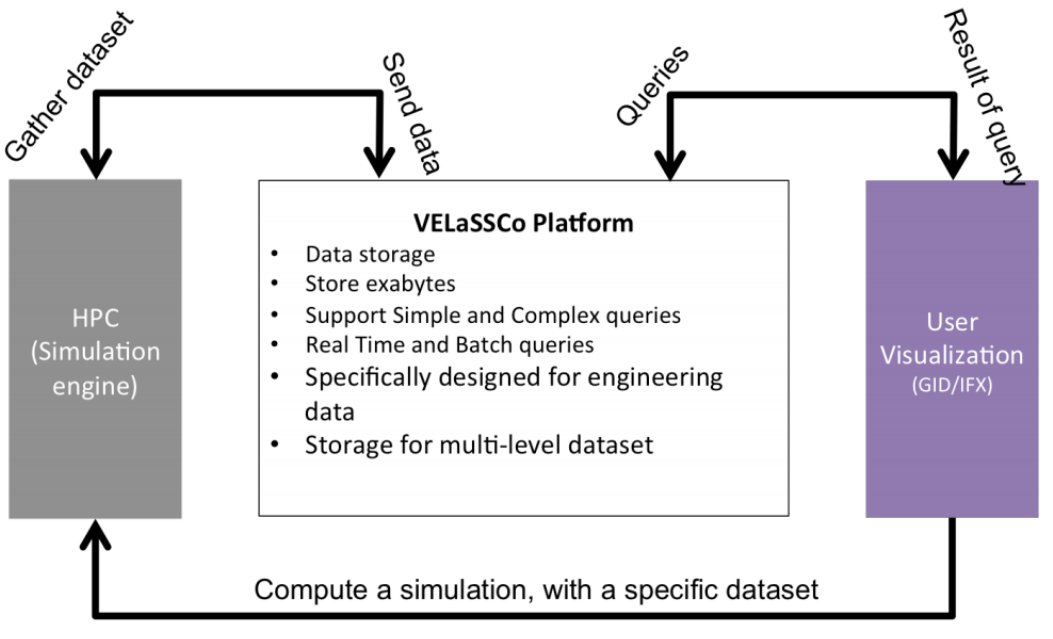
\includegraphics[width=\textwidth]{images/vel}
	\caption{Interazione di \textit{VELaSSCo} con i moduli di calcolo e simulazione e quelli di visualizzazione.}
	\label{fig:vel}
\end{figure}
Il design di \textit{VELaSSCo} (Figura \ref{fig:vel}) è incentrato su tre macro componenti principali.
\begin{description}
	\item [Data Layer] Si occupa dello storage e dell'organizzazione fisica dei dati all'interno della macchina distribuita. E' basato sull'utilizzo di database distribuiti come HBase .
	\item [Data Analytics Layer] Si occupa dell'analisi dei dati. E' implementato seguendo il paradigma map-reduce  ed è ciò che rende la piattaforma estremamente scalabile, estensibile e generale. Moduli analitici esterni scritti da terze parti possono essere facilmente integrati all'interno del sistema per fare fronte alle esigenze analitiche dell'analisi e/o simulazione previste.
	\item [Visualization Layer] 
	Questo modulo ha l'obiettivo di rendere possibile la visualizzazione 2-3/D dei dati e l'interazione con il modulo di analytics.
\end{description}
Il workflow tipico nell'ambito del calcolo scientifico prevede
\begin{inparadesc}
	\item[l'esecuzione] del solver o modello di simulazione in un HPC, il
	\item[salvataggio]  dati su disco ed infine il
	\item[trasferimento] dei dati dall'HPC al client di visualizzazione ed analisi.
\end{inparadesc}
Storicamente un approccio di questo tipo ha avuto successo principalmente perché l'hardware grafico e di calcolo erano completamente separati e differenze tra velocità di calcolo e scrittura su disco erano relativamente piccole.
Tuttavia, dopo l'avvento della GPGPU, la distinzione netta tra HW grafico e
HW di calcolo è stata drasticamente diminuita, ed il divario tra velocità dei processori e quella dei dispositivi di storage permanente è arrivato ad essere di almeno di due ordini di grandezza.
Ad aggravare la situazione di inadeguatezza del workflow tipico vanno ad aggiungersi che l'avvento delle tecnologie che vanno sotto al nome di Big-Data  hanno fatto si che solvers siano in grado di produrre quantità di dati impensabili fino a pochi anni fa (soprattutto nel campo dell'ingegneria e della fisica). 
\begin{figure}[!htbp]
	\centering
	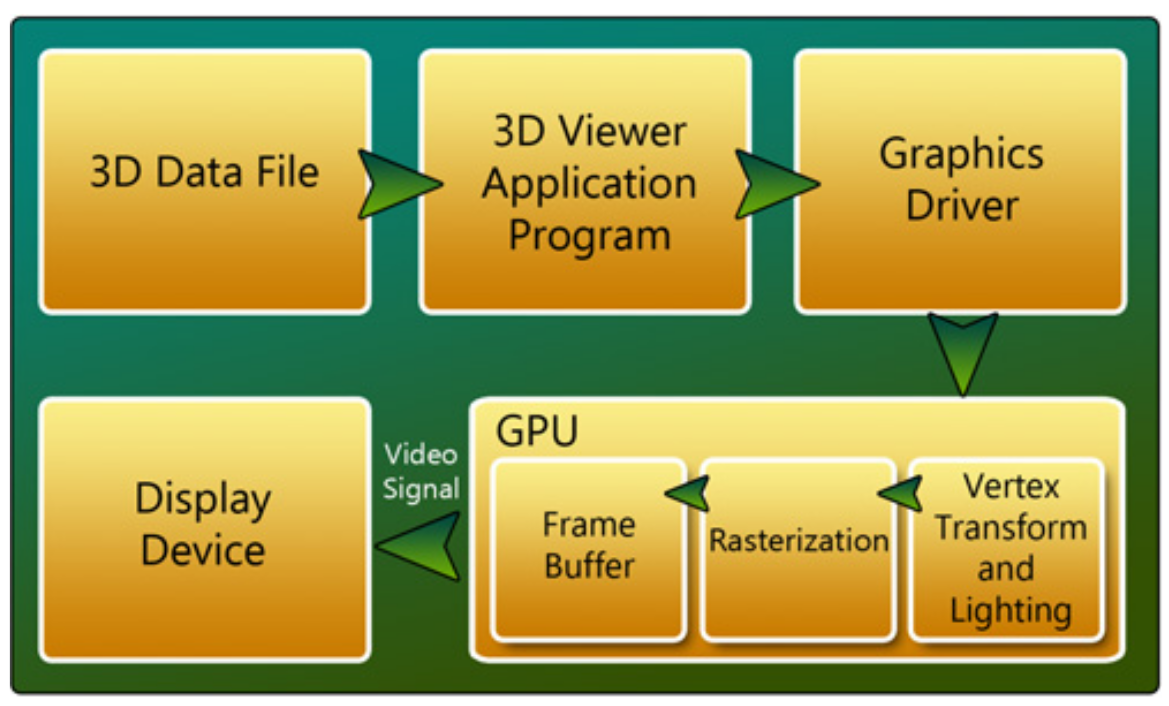
\includegraphics[scale=0.3]{images/pipeline}
	\caption{Schematizzazione della pipeline grafica.}
	\label{fig:pip}
\end{figure}
Obiettivo del mio periodo di ricerca (Novembre 2015-Luglio 2016) presso la \textit{University of Edinburgh} era quello progettare ed implementare un primo prototipo per risolvere il problema della visualizzazione interattiva all'interno di \textit{VELaSSCo}. La soluzione proposta è  quella dell'applicazione del offline rendering parallelo.
Durante il processo di rendering i dati RAW vengono trasformati  all'interno della pipeline grafica (Figura \ref{fig:pip}) fino ad arrivare in ultima istanza ad essere quello che è un sottoprodotto grafico direttamente visualizzabile dalle schede grafiche, il frame-buffer la cui  dimensione è relativamente piccola (decine di MB nel peggiori dei casi).
L'idea è quella che tutto il processing grafico avvenga in remoto direttamente sulle macchine che fanno HPC e che l'analista riceva solamente i framebuffers.
Queste idee sono state
La soluzione proposta è stata quella di:
\begin{itemize}
	\item progettare ed implementare un layer di rendering parallelo
	\item dotare la piattaforma di un numero di nodi dedicati al processing grafico (il cui numero è determinato in base al carico massimo del sistema, al numero di utenti connessi simultaneamente etc.)
	
\end{itemize}

Il processo di rendering può essere visto come un problema di ordinamento delle primitive grafiche sulla superificie dello schermo. In un renderer parallelo questo sorting richiede la ridistribuzione delle primitive tra tutti i processori perché la responsabilità per il rendering dello schermo è condivisa.
Esistono principalmente tre tipi di rendering parallelo, \textit{Sort First, Sort Middle} e \textit{Sort Last}; ognuno di essi differisce dagli altri per il momento in cui questa suddivisione avviene. Teoricamente essa può avvenire in qualunque istante durante l'esecuzione della pipeline grafica (Figure \ref{fig:sl} e \ref{fig:sfsm}).


\begin{figure}[!htbp]
	\centering
	\begin{minipage}{0.4\textwidth}
		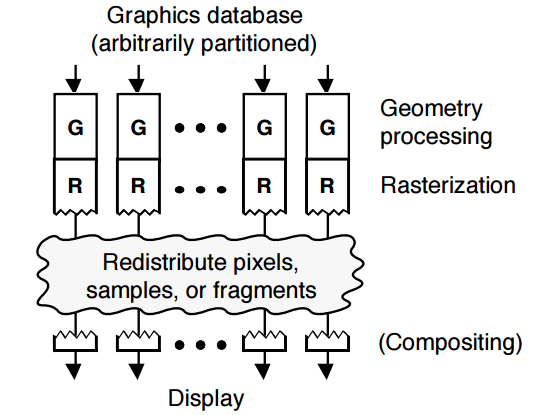
\includegraphics[scale=0.28]{images/sortlatst}
		\label{fig:sf}
	\end{minipage}
	\hfill
	\begin{minipage}{0.5\textwidth}
		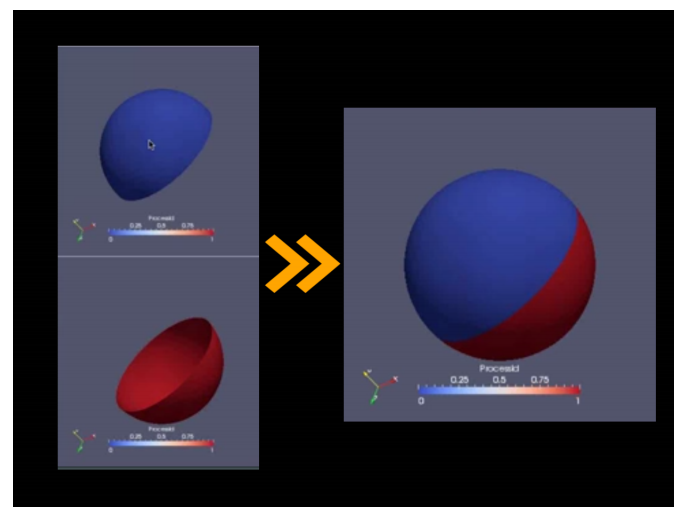
\includegraphics[scale=0.28]{images/sortlastex}
	\end{minipage}
	\caption{Sort-last. Esempio di composizione finale del framebuffer.}\label{fig:sl}
\end{figure}

Il prototipo sviluppato è di tipo sort-last, poiché questa strategia è l'unica che non suddivide le primitive in base alla porzione di schermo che modificano.
Il set di primitive grafiche viene suddiviso tra i processori secondo una policy che garantisce il load balancing (ogni processore può calcolare primitive che modificano qualunque parte dello schermo) e in fase di rastering tutti i risultati intermedi vengono \textit{ricomposti} a formare un unico framebuffer. La composizione avviene tenendo in considerazione lo z-buffer (Figura \ref{fig:sl}).

Il primo prototipo implementato ha mostrato ottimi risultati in termini di numero di primitive per secondo eseguite ed è in grado di effettuare il rendering di dati su schermi ad altissima risoluzione (schermi compositi). 



\begin{figure}[!htbp]
	\centering
	\begin{minipage}{0.4\textwidth}
		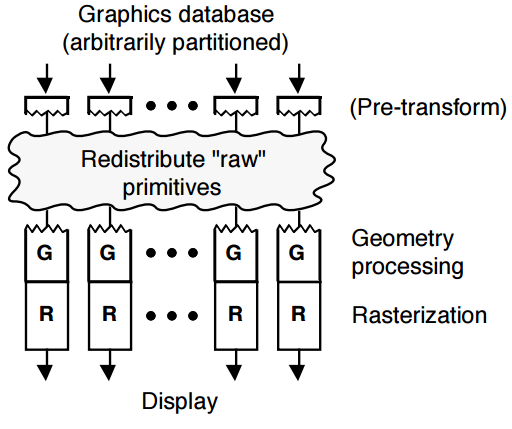
\includegraphics[scale=0.28]{images/sortfirst}      
		\label{fig:sf}
	\end{minipage}
	\hfill
	\begin{minipage}{0.4\textwidth}
		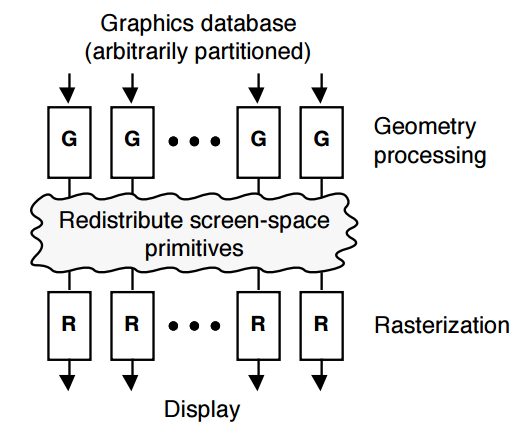
\includegraphics[scale=0.28]{images/sortmiddle}
		\label{fig:sm}
	\end{minipage}
	\caption{Sort first and Sort middle rendering.}\label{fig:sfsm}
\end{figure}


\subsection{Particle-like Objects Tracking}
\definecolor{myblue}{RGB}{80,80,160}
\definecolor{mygreen}{RGB}{80,160,80}
\begin{figure}[!htbp]
	\centering
	\begin{tikzpicture}[thick,
	every node/.style={draw,circle},
	fsnode/.style={fill=gray!30},
	ssnode/.style={fill=gray!90},
	every fit/.style={ellipse,inner sep=-2pt,text width=cm},
	->,shorten >= 3pt,shorten <= 3pt
	]
	
	% the vertices of Frame1
	\begin{scope}[start chain=going below,node distance=5mm, every node/.style={circle,minimum size=3.35em}]
	
	\node[fsnode,on chain,label=above:$\boldsymbol{M_{i}}$] (f0)  {$p^i_1$};
	\node[fsnode,on chain] (f1)  {$p^i_2$};
	
	\node[below of=f1,node distance=10,yshift=-10] {$\vdots$};
	
	\node[fsnode,on chain] (f2)  {$p^i_{j}$};
	\node[below of=f2,node distance=10,yshift=-10] {$\vdots$};
	\node[fsnode,on chain] (fl)  {$p^{i}_l$};
	\node[below of=fl,node distance=10,yshift=-10] {$\vdots$};
	
	\node[fsnode,on chain] (f3) {$p^i_n$};
	\end{scope}
	
	% the vertices of Frame1
	\begin{scope}[xshift=6cm,start chain=going below,auto, every node/.style={circle,minimum size=3.3em},node distance=5mm]
	
	\node[ssnode,on chain,label=above:$\boldsymbol{P_{i+1}}$] (s0)  {$p^{i+1}_1$};
	\node[ssnode,on chain] (s1)  {$p^{i+1}_2$};
	\node[draw=none,below of=s1,node distance=10,yshift=-10] {$\vdots$};
	
	\node[ssnode,on chain] (sk)  {$p^{i+1}_k$};
	\node[draw=none,below of=sk,node distance=10,yshift=-10] {$\vdots$};
	\node[ssnode,on chain] (s2)  {$p^{i+1}_{m-1}$};
	\node[ssnode,on chain] (s3)  {$p^{i+1}_m$};
	\end{scope}
	% the set U
	
	\node [myblue,draw=none] {};
	% the set V
	\node [mygreen,draw=none] {};
	\begin{scope}[every edge/.style={draw,thin}]
	% the edges
	\draw (f0) edge[red, thick, dashed]  (s3);
	\foreach \i in {0}
	\foreach \j in {0,1,2}
	\draw (f\i) edge  (s\j);
	
	
	\draw (f1) edge[red,thick, dashed]  (s0);
	\foreach \i in {1}
	\foreach \j in {1,2,3}
	\draw (f\i) edge  (s\j);
	
	\draw (f2) edge[red, thick,dashed]  (s1);
	\foreach \i in {2}
	\foreach \j in {0,2,3}
	\draw (f\i) edge  (s\j);
	
	\draw (f3) edge[red, thick,dashed]  (s2);
	\foreach \i in {3}
	\foreach \j in {1,3,0}
	\draw (f\i) edge  (s\j);

	\end{scope}
	
	\end{tikzpicture}
	\caption{}
	\label{match}
\end{figure}
Il tracking di oggetti microscopici svolge un ruolo molto importante in molti ambiti scientifici per lo studio del movimento di particelle,  micro-sfere   e nanoparticelle. In particolare lo studio delle traiettorie che questi oggetti assumono è importante per calcolarne proprietà cinametiche e dinamiche. Vengono frequentemente utilizzate tecniche semi-automatiche per il tracking, ma questo approccio non è efficace quando il numero di particelle è grande.
Ho sviluppato quindi un software basato sul paradigma degli automi cellulari estesi (XCA) che è in grado di ricostruire le traiettorie di questo tipo di oggetti in modo automatico ed ho lavorato congiuntamente con alcuni ricercatori dell'istituto di BioEngineering dell'Università di Edimburgo per l'applicazione di questo software ad un caso di studio reale: il tracking del batterio \textit{B.subtilis} in un dispositivo microfiudico.

L'algoritmo sviluppato è in grado di produrre un set di traiettorie $ T_n = \{ t_i \}$  s.t.  $t_i=\{ c^i_k,c^i_{k+1},\ldots,c^i_l \} $ a partire da un insieme di input di particelle $P=P_1 \cup P_2 \cup \ldots \cup P_n$ e una funzione $\mathcal{D} :  P \times P \mapsto \mathbb{R}$, 
la funzione  \textit{distanza}.
$P_i = \{p^j_i \; | \; 1 \leq j\; \}$ sono tutte le particelle al tempo $i$ e ogni particella $p_i^j$ è definita da un centroide, un bounding box che ne descrive le proprietà geometriche e spaziali. 
$\mathcal{D}(p,q)$ misura quanto è probabile che  $p$ sia stata trasformata in $q$ dopo l'applicazione di zero o più trasformazioni geometriche (scaling, traslazione, rotazione, shearing etc.). 

L'algoritmo ad ogni step processa un frame $P_i$ ed un set di traiettorie parziali $M_i$ cercando di trovare un match ta le particelle in $P_i$ ed una traiettorie in $M_i$ e può essere ridotto ad una variante del problema dell'assegnamento in un grafo bipartito.
Più specificatamente l'algoritmo consiste nel trovare un matching di peso minimo (non necessariamente perfetto) in un grafo bipartito diretto e pesato $G=(V,E)$ dove $V={M_i} \cup P_i$ è il set di nodi ${M_i}, P_i$ sono le due partizioni, $E = {M_i} \times P_i$ t.c. $e \in E, \mathcal{D}(e) \in \mathbb{R}$ sia il peso dell'arco $e$.
Un matching valido deve soddisfare i seguenti constraints: 
\begin{equation}
\forall (u,v) \in S 
\left\{
\begin{array}{lr}
(w,x) \in S,\; v=x\Longleftrightarrow u=w\\
\mathcal{D}(u,v) = \min_{x \in V_2} \mathcal{D}(u,x)  \\
\nexists \: (w,v) \in E \: \mbox{s.t.} \: \mathcal{D}(w,v) < \mathcal{D}(u,v)
\end{array}
\right.
\label{matchConstraints}
\end{equation}
\begin{figure}[!htbp]
	\begin{minipage}[l]{0.5\textwidth}
		\centering
		
\includegraphics[width=5.5cm]{images/bacteriasmall}
		\caption{Immagine Raw di input. I Batteri appaio come cluster neri mentre grigio e bianco rappresentano rumore di fondo e abberazioni cromatiche dovute all'interazione della luce con il materiale del dispositivo microfluidico. } \label{AAA}
	\end{minipage}   
	\hfill{}
	\begin{minipage}[r]{0.5\textwidth}
		\centering
		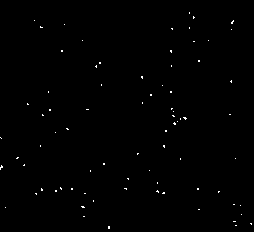
\includegraphics[width=5.5cm]{images/bacteriasmall_threshold}
		\caption{Immagine binaria ottenuta applicando filtri di threshold, constrast stretching e convoluzione gaussiana utilizzando il framework presentato. Rumore e backgraound sono stati eliminati, segmentando correttamente i batteri.} \label{BBB}
	\end{minipage}
\end{figure}
Se denotiamo  l'operatore di match utilizzando la seguente relazione di ricorrenza $  M_i \lozenge P_{i+1} = (T_{i+1},M_{i+1}) $, $M_0=P_0$, l'intera procedura può essere riscritta come $(T_n,M_n) = M_{n-1} \lozenge P_{n}=(((P_0 \lozenge P_1)\lozenge P_2) \lozenge \ldots \lozenge P_n)$.
Attualmente il lavoro che sto svolgendo è dimostrare che l'operatore $\lozenge $ è associativo, e sotto questa ipotesi la medesima procedura è immediatamente parallelizzabile utilizzando il paradigma della parallel reduction.

La Figura \ref{match} mostra un'applicazione dell'operatore $\lozenge$ al frame $P_{i+1}$ composto da $m$ particles. Le linee rosse tratteggiate mostrano la soluzione $S$.
Supponiamo ad esempio che esista una traiettoria in $M_i$, $t_*=p^s_a \leadsto p^i_1$ . Essa verrà ulteriormente allungata dal match trovato da $\lozenge$ con la particella $p^{i+1}_m$ diventando $t=p^s_a \leadsto p^i_1 \to p^{i+1}_m$.

Un framework basato sugli automi cellulari estesi che è in grado di effettuare operazioni di image processing su dati $n$-dimensionali come ad esempio la convoluzioni è stato sviluppato. Questo framework è intrinsecamente parallelo e può essere eseguito su diverse architetture parallele (una versione per macchine a memoria condivisa è già disponibile). Un esempio di utilizzo di tale framework è dato dalle Figure \ref{AAA} e \ref{BBB}.

I risultati ottenuti sono molto promettenti in quanto siamo stato in grado di calcolare alcuni parametri riguardanti il moto del batterio \textit{B. subtilis}, come il tempo di \textit{tumble} medio e la velocità di \textit{run}. 
Tutti i risultati sono in accordo con i valori standard trovati in letteratura, a conferma che le traiettorie sono ricostruite con buona precisione (Figura \ref{fig:res}).

\begin{figure}[!htbp]
	\begin{center}
		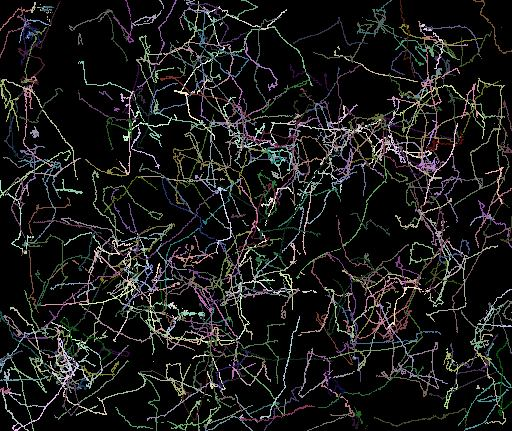
\includegraphics[scale=0.75]{images/result.png}
		\caption{Traiettorie traccate utilizzando un filmato time-lapse di 4100 frames. Per rendere più chiara l'immagine un colore random è associato ad ogni traiettoria.}\label{fig:res}
	\end{center}
\end{figure}
